% --- Template for thesis / report with tktltiki2 class ---
% 
% last updated 2013/02/15 for tkltiki2 v1.02
\documentclass[finnish]{tktltiki2}
%\usepackage[finnish]{babel}
%\usepackage[utf8x]{inputenc}

% tktltiki2 automatically loads babel, so you can simply
% give the language parameter (e.g. finnish, swedish, english, british) as
% a parameter for the class: \documentclass[finnish]{tktltiki2}.
% The information on title and abstract is generated automatically depending on
% the language, see below if you need to change any of these manually.
% 
% Class options:
% - grading                 -- Print labels for grading information on the front page.
% - disablelastpagecounter  -- Disables the automatic generation of page number information
%                              in the abstract. See also \numberofpagesinformation{} command below.
%
% The class also respects the following options of article class:
%   10pt, 11pt, 12pt, final, draft, oneside, twoside,
%   openright, openany, onecolumn, twocolumn, leqno, fleqn
%
% The default font size is 11pt. The paper size used is A4, other sizes are not supported.
%
% rubber: module pdftex

% --- General packages ---
\usepackage[utf8]{inputenc}
\usepackage[T1]{fontenc}
\usepackage{lmodern}
\usepackage{microtype}
\usepackage{amsfonts,amsmath,amssymb,amsthm,booktabs,color,enumitem,graphicx}
\usepackage[pdftex,hidelinks]{hyperref}
\usepackage{apacite}
\usepackage{hyperref}
\usepackage{minted}
\usepackage{listings}
\usemintedstyle{vs}

% Automatically set the PDF metadata fields
\makeatletter
\AtBeginDocument{\hypersetup{pdftitle = {\@title}, pdfauthor = {\@author}}}

\renewcommand{\lstlistingname}{Esimerkki}

\usepackage{color}
\definecolor{lightgray}{rgb}{0.95, 0.95, 0.95}
\definecolor{darkgray}{rgb}{0.4, 0.4, 0.4}
%\definecolor{purple}{rgb}{0.65, 0.12, 0.82}
\definecolor{editorGray}{rgb}{0.95, 0.95, 0.95}
\definecolor{editorOcher}{rgb}{1, 0.5, 0} % #FF7F00 -> rgb(239, 169, 0)
\definecolor{editorGreen}{rgb}{0, 0.5, 0} % #007C00 -> rgb(0, 124, 0)
\definecolor{orange}{rgb}{1,0.45,0.13}		
\definecolor{olive}{rgb}{0.17,0.59,0.20}
\definecolor{brown}{rgb}{0.69,0.31,0.31}
\definecolor{purple}{rgb}{0.38,0.18,0.81}
\definecolor{lightblue}{rgb}{0.1,0.57,0.7}
\definecolor{lightred}{rgb}{1,0.4,0.5}
\usepackage{upquote}
\usepackage{listings}
% CSS
\lstdefinelanguage{CSS}{
  keywords={color,background-image:,margin,padding,font,weight,display,position,top,left,right,bottom,list,style,border,size,white,space,min,width, transition:, transform:, transition-property, transition-duration, transition-timing-function},	
  sensitive=true,
  morecomment=[l]{//},
  morecomment=[s]{/*}{*/},
  morestring=[b]',
  morestring=[b]",
  alsoletter={:},
  alsodigit={-}
}

% JavaScript
\lstdefinelanguage{JavaScript}{
  morekeywords={typeof, new, true, false, catch, function, return, null, catch, switch, var, if, in, while, do, else, case, break},
  morecomment=[s]{/*}{*/},
  morecomment=[l]//,
  morestring=[b]",
  morestring=[b]'
}

\lstdefinelanguage{HTML5}{
  language=html,
  sensitive=true,	
  alsoletter={<>=-},	
  morecomment=[s]{<!-}{-->},
  tag=[s],
  otherkeywords={
  % General
  >,
  % Standard tags
	<!DOCTYPE,
  </html, <html, <head, <title, </title, <style, </style, <link, </head, <meta, />,
	% body
	</body, <body,
	% Divs
	</div, <div, </div>, 
	% Paragraphs
	</p, <p, </p>,
	% scripts
	</script, <script,
  % More tags...
  <canvas, /canvas>, <svg, <rect, <animateTransform, </rect>, </svg>, <video, <source, <iframe, </iframe>, </video>, <image, </image>, <header, </header, <article, </article
  },
  ndkeywords={
  % General
  =,
  % HTML attributes
  charset=, src=, id=, width=, height=, style=, type=, rel=, href=,
  % SVG attributes
  fill=, attributeName=, begin=, dur=, from=, to=, poster=, controls=, x=, y=, repeatCount=, xlink:href=,
  % properties
  margin:, padding:, background-image:, border:, top:, left:, position:, width:, height:, margin-top:, margin-bottom:, font-size:, line-height:,
	% CSS3 properties
  transform:, -moz-transform:, -webkit-transform:,
  animation:, -webkit-animation:,
  transition:,  transition-duration:, transition-property:, transition-timing-function:,
  }
}

\lstdefinestyle{htmlcssjs} {%
  % General design
%  backgroundcolor=\color{editorGray},
  basicstyle={\footnotesize\ttfamily},   
  frame=b,
  % line-numbers
  xleftmargin={0.75cm},
  numbers=left,
  stepnumber=1,
  firstnumber=1,
  numberfirstline=true,	
  % Code design
  identifierstyle=\color{black},
  keywordstyle=\color{blue}\bfseries,
  ndkeywordstyle=\color{editorGreen}\bfseries,
  stringstyle=\color{editorOcher}\ttfamily,
  commentstyle=\color{brown}\ttfamily,
  % Code
  language=HTML5,
  alsolanguage=JavaScript,
  alsodigit={.:;},	
  tabsize=2,
  showtabs=false,
  showspaces=false,
  showstringspaces=false,
  extendedchars=true,
  breaklines=true,
  % German umlauts
  literate=%
  {Ö}{{\"O}}1
  {Ä}{{\"A}}1
  {Ü}{{\"U}}1
  {ß}{{\ss}}1
  {ü}{{\"u}}1
  {ä}{{\"a}}1
  {ö}{{\"o}}1
}
%
\lstdefinestyle{py} {%
language=python,
literate=%
*{0}{{{\color{lightred}0}}}1
{1}{{{\color{lightred}1}}}1
{2}{{{\color{lightred}2}}}1
{3}{{{\color{lightred}3}}}1
{4}{{{\color{lightred}4}}}1
{5}{{{\color{lightred}5}}}1
{6}{{{\color{lightred}6}}}1
{7}{{{\color{lightred}7}}}1
{8}{{{\color{lightred}8}}}1
{9}{{{\color{lightred}9}}}1,
basicstyle=\footnotesize\ttfamily, % Standardschrift
numbers=left,               % Ort der Zeilennummern
%numberstyle=\tiny,          % Stil der Zeilennummern
%stepnumber=2,               % Abstand zwischen den Zeilennummern
numbersep=5pt,              % Abstand der Nummern zum Text
tabsize=4,                  % Groesse von Tabs
extendedchars=true,         %
breaklines=true,            % Zeilen werden Umgebrochen
keywordstyle=\color{blue}\bfseries,
frame=b,
commentstyle=\color{brown}\itshape,
stringstyle=\color{editorOcher}\ttfamily, % Farbe der String
showspaces=false,           % Leerzeichen anzeigen ?
showtabs=false,             % Tabs anzeigen ?
xleftmargin=17pt,
framexleftmargin=17pt,
framexrightmargin=5pt,
framexbottommargin=4pt,
%backgroundcolor=\color{lightgray},
showstringspaces=false,      % Leerzeichen in Strings anzeigen ?
}%

\makeatother

% --- Language-related settings ---
%
% these should be modified according to your language

% babelbib for non-english bibliography using bibtex
\usepackage[fixlanguage]{babelbib}
\selectbiblanguage{finnish}

% add bibliography to the table of contents
\usepackage[nottoc]{tocbibind}
% tocbibind renames the bibliography, use the following to change it back
\settocbibname{Lähteet}

% --- Theorem environment definitions ---

\newtheorem{lau}{Lause}
\newtheorem{lem}[lau]{Lemma}
\newtheorem{kor}[lau]{Korollaari}

\theoremstyle{definition}
\newtheorem{maar}[lau]{Määritelmä}
\newtheorem{ong}{Ongelma}
\newtheorem{alg}[lau]{Algoritmi}
\newtheorem{esim}[lau]{Esimerkki}

\theoremstyle{remark}
\newtheorem*{huom}{Huomautus}

% --- tktltiki2 options ---
%
% The following commands define the information used to generate title and
% abstract pages. The following entries should be always specified:

\title{Angular web-sovelluskehys}
\author{Eveliina Pakarinen, 014152724}
\date{\today}
\level{Ohjelmistoarkkitehtuurien harjoitustyö}
\abstract{Tiivistelmä}

% The following can be used to specify keywords and classification of the paper:

\keywords{avain, sanat}

% classification according to ACM Computing Classification System (http://www.acm.org/about/class/)
% This is probably mostly relevant for computer scientists
% uncomment the following; contents of \classification will be printed under the abstract with a title
% "ACM Computing Classification System (CCS):"
% \classification{}

% If the automatic page number counting is not working as desired in your case,
% uncomment the following to manually set the number of pages displayed in the abstract page:
%
% \numberofpagesinformation{16 sivua + 10 sivua liitteissä}
%
% If you are not a computer scientist, you will want to uncomment the following by hand and specify
% your department, faculty and subject by hand:
%
% \faculty{Matemaattis-luonnontieteellinen}
% \department{Tietojenkäsittelytieteen laitos}
% \subject{Tietojenkäsittelytiede}
%
% If you are not from the University of Helsinki, then you will most likely want to set these also:
%
% \university{Helsingin Yliopisto}
% \universitylong{HELSINGIN YLIOPISTO --- HELSINGFORS UNIVERSITET --- UNIVERSITY OF HELSINKI} % displayed on the top of the abstract page
% \city{Helsinki}
%
\usepackage{float}
\usepackage{graphicx}

\addtolength{\oddsidemargin}{-.5in}
\addtolength{\evensidemargin}{-.5in}
\addtolength{\textwidth}{1in}
\addtolength{\topmargin}{-.5in}
\addtolength{\textheight}{1in}
\numberwithin{figure}{section}

\begin{document}

% --- Front matter ---

\frontmatter      % roman page numbering for front matter

\maketitle        % title page
% \makeabstract     % abstract page

\tableofcontents  % table of contents

% --- Main matter ---

\mainmatter       % clear page, start arabic page numbering

\setlength{\parindent}{2.5em}
\setlength{\parskip}{0em}
\renewcommand{\baselinestretch}{1.5}
\large

\section{Johdanto}

Angular on asiakaspuolen web-sovelluskehys ja -sovellusalusta, jonka avulla voidaan toteuttaa asiakaspuolen web-ohjelmistoja \cite{ArchitectureOverview}. Tässä harjoitustyössä käsitellään Angularia versiopäivityksen 2.0 jälkeen. Harjoitustyön kirjoittamishetkellä viimeisin Angularin pääversio on Angular 6.0.

Angularin arkkitehtuurityylejä ovat modulaarisuus ja komponenttipohjaisuus \cite{ArchitectureModules,ArchitectureComponents}. Angularissa on oma modulaarisuusjärjestelmä. Angularin moduulit koostuvat komponenteista. Angular toteuttaa myös useita ohjelmistotason ratkaisumalleja kuten riippuvuusinjektion ja yhdensuuntaisen tiedonsiirron.

% \newpage

\section{Kehyksen esittely}

Angular on asiakaspuolen web-sovelluskehys ja -sovellusalusta, jonka avulla voidaan toteuttaa asiakaspuolen web-ohjelmistoja \cite{ArchitectureOverview}. Angular on toteutettu TypeScript-ohjelmointikielellä kirjastoina, joista Angularin ydin ja valinnaiset osat koostuvat ja joiden pohjalta voidaan koostaa uusia sovelluksia.    

\subsection{Arkkitehtuurityylit ja komponenttien roolijako}

Angular-sovelluskehyksellä toteutetut sovellukset koostuvat useasta eri pääosasta, joita ovat \textit{moduulit} (\textit{modules}), \textit{komponentit} (\textit{components}) ja \textit{palvelut} (\textit{services}) \cite{ArchitectureOverview}. Näiden osien välisiä suhteita kuvataan kuvassa \ref{fig:AngularAppArchitectureOverview}. 

Yksi Angularin arkkitehtuurityyleistä on modulaarisuus. Modulaarisuus on toteutettu Angularissa modulaarisuusjärjestelmällä \textit{NgModules} \cite{ArchitectureModules}. Moduuleilla voidaan kapseloida yhtenäiseksi kokonaisuudeksi yksi toiminnallinen kokonaisuus. Angular-sovellukset koostuvat yhdestä tai useammasta NgModule-moduulista. Jokaisessa Angular-sovelluksessa on vähintään yksi NgModule-luokka juurimoduulina \cite{ArchitectureModules}. 

Moduuleihin voidaan myös tuoda lisää toiminnallisuutta importoimalla muita NgModuuleja \cite{ArchitectureModules}. Lisäksi moduulista voidaan exportoida toiminnallisuutta, jotta sitä voidaan käyttää muissa moduuleissa hyödyksi. Juurimoduuli ja moduulien importoiminen ja exportoiminen on kuvattu kuvassa \ref{fig:AngularAppArchitectureOverview} sinisillä laatikoilla ja nuolilla.

Toinen Angularin arkkitehtuurityyleistä on komponenttipohjaisuus. Angular-moduulit koostuvat komponenteista, joita voi olla yhdessä moduulissa yksi tai useampia \cite{ArchitectureModules}. Jokaiseen juurimoduuliin sisältyy juurikomponentti, joka on kuvattu kaaviossa \ref{fig:AngularAppArchitectureOverview} vihreällä laatikolla. Angular-komponenttien tarkoitus on määritellä yksi osa ruudulla näkyvästä sisällöstä ja kontrolloida sen toiminnallisuutta \cite{ArchitectureComponents}. Komponentit koostuvat komponenttiin liittyvästä sovelluslogiikasta ja komponenttiin liittyvästä \textit{templaatista} (\textit{template}). Komponenttiin liittyvä sovelluslogiikka määritellään komponentin TypeScript-luokassa. Kuvassa \ref{fig:AngularAppArchitectureOverview} templaatit on kuvattu komponenttien sisään keltaisilla laatikoilla. 

Yhdessä komponenttilogiikka ja komponenttiin liittyvä templaatti määrittelevät \textit{näkymän} (\textit{view}) \cite{ArchitectureModules}. Näkymät ovat sovelluksessa yksittäisiä osia, jotka kontrolloivat yhtä osaa ruudulla näkyvästä sisällöstä \cite{ArchitectureComponents}. Näkymät voivat muodostaa puumaisen hierarkian, sillä näkymissä voidaan viitata toisiin näkymiin sekä saman moduulin sisällä että importoiduissa moduuleissa \cite{ArchitectureModules}. 

Templaatit toteutetaan HTML-kielellä ja Angularin omalla templaatti syntaksilla, jonka avulla HTML-rakennetta voidaan muuttaa sovelluslogiikan perusteella \cite{ArchitectureComponents}. Templaateissa voidaan käyttää \textit{direktiivejä} (\textit{directive}) sovelluslogiikan tuomiseen templaattiin \cite{TemplateSyntax}. Kuvassa \ref{fig:AngularAppArchitectureOverview} direktiivistä esimerkkinä toimii \mintinline{JavaScript}{*ngIf}, joka löytyy liilasta laatikosta juuritemplaatti-laatikon sisältä. 

\textit{Datasidonnan} (\textit{data binding}) avulla yhdistetään templaatissa DOM-mallissa näytettävä data ja komponentin sovelluslogiikassa käsiteltävä data toisiinsa \cite{ArchitectureComponents}. Templaatissa käytettävästä datasidontasyntaksista kuvassa \ref{fig:AngularAppArchitectureOverview} esimerkkeinä toimivat \mintinline{JavaScript}{[user]}, \mintinline{JavaScript}{(click)}, \mintinline{JavaScript}{[(ngModel)]} ja \mintinline{JavaScript}{{{user.name}}}. Toisiin komponentteihin viittaamisesta kuvassa \ref{fig:AngularAppArchitectureOverview} esimerkkinä toimii HTML-tagi \mintinline{JavaScript}{<app-user-detail>}.

Yksi Angularin modulaarisuutta ja uudelleenkäytettävyyttä tukeva piirre on erottaa palvelut komponenteista \cite{ArchitectureServices}. Palvelut ovat luokkia, joiden avulla voidaan toteuttaa yksi hyvin määritelty sovelluksen tarvitsema toiminnallisuus. Kuvassa \ref{fig:AngularAppArchitectureOverview} palvelut on kuvattu punaisilla laatikoilla. Palveluita voidaan injektoida komponentteihin riippuvuuksina \cite{ArchitectureServices}. 


\begin{figure}[H]
  \centering
  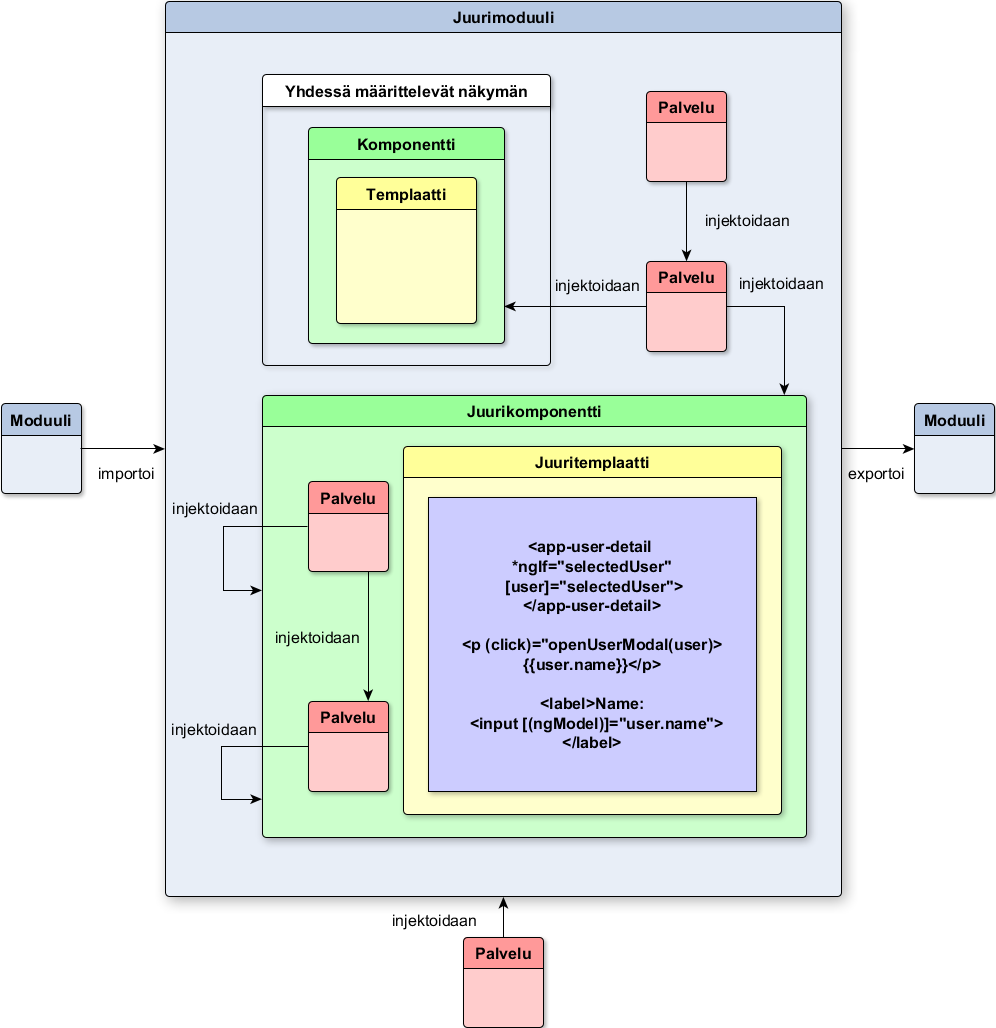
\includegraphics[width=14cm]{images/AngularAppArchitectureOverview.png}
  \caption{Angular-sovelluskehyksen pääosien suhteet toisiinsa}
  \label{fig:AngularAppArchitectureOverview}
\end{figure}

\section{Kehyksen yleiskuva}

Angular web-sovelluskehys pohjautuu modulaariseen komponenttipohjaiseen arkkitehtuurityyliin. Angular toteuttaa kuitenkin myös useita ohjelmistotason ratkaisumalleja, joita ovat esimerkiksi riippuvuusinjektio, yhdensuuntainen tiedonsiirto ja reaktiivinen ohjelmointi.

\subsection{Ohjelmistotason ratkaisumallit}

Yksi Angularissa sovellettavista ohjelmistotason ratkaisumalleista on \textit{riippuvuusinjektio} (\textit{dependency injection}), jonka avulla komponenteille voidaan tuoda käyttöön niiden tarvitsemaa lisätoiminnallisuutta \cite{DependencyInjectionPattern}. Angularissa riippuvuusinjektion avulla komponenteille voidaan tarjota palveluissa toteutettua uudelleenkäytettävää toiminnallisuutta. Palvelut voidaan injektoida niin, että palvelun näkyvyysalue on koko sovelluksen laajuisesti, tietyn moduulin sisällä tai tietyn komponentin sisällä \cite{DependencyInjection}. Palveluiden näkyvyysalueet tulevat esiin myös kuvasta \ref{fig:AngularAppArchitectureOverview} punaisten palvelu-laatikoiden sijoittelusta moduuli- ja komponenttilaatikoiden sisä- ja ulkopuolelle.

Toinen Angularissa sovellettavista ratkaisumalleista on \textit{yhdensuuntainen tiedonsiirto} (\textit{unidirectional data flow}). Angularissa DOM-mallissa näytettävä data ja komponentin sovelluslogiikassa käsiteltävä data yhdistetään toisiinsa datasidonnan avulla \cite{TemplateSyntax}. Datasidontaa on kolmea eri tyyppiä: datan lähteeltä näkymää kohti (\textit{source-to-view}), näkymästä datan lähdettä kohti (\textit{view-to-source}) ja kahdensuuntainen datasidonta (\textit{view-to-source-to-view}), joka on yhdistelmä kahdesta ensin mainitusta datasidontatyypistä \cite{TemplateSyntax}. 

Datasidonnan avulla näkymään sisältyvät templaatti ja komponentti voivat välittää tietoa toisilleen \cite{ArchitectureComponents}. Lisäksi Angular-sovelluksen puumaisen rakenteen vanhempi- ja lapsikomponentti voivat välittää tietoa toisilleen datasidonnan avulla \cite{ArchitectureComponents}. Datasidonnalla on siis tärkeä merkitys sovelluksen sisäisten osien kommunikaation kannalta \cite{ArchitectureComponents}. Kahdensuuntaisessa datasidonnassa syötekenttä voi saada lähtöarvon komponentilta \textit{source-to-view}-sidonnan avulla ja käyttäjän tekemän muutoksen jälkeen muuttunut sisältö päivittyy takaisin komponentille \textit{view-to-source}-sidonnalla. 

TODO: Reaktiivinen ohjelmointi!!!!!!!!!!!!!!! Observable-datavirta, käytössä Angularin coressa, ajaxin sijaan (??) \textit{Mika: Reaktiivisuuden huono puoli --> jos on paljon riippuvuuksia ja kuuntelee streameja voi tapahtua omituisia asioita toisessa palvelussa kun toinen palvelu ehtinyt jo muuttaa tilaa}

\subsection{Sovelluskohtainen erikoistaminen}

Angular-sovelluskehyksellä toteutettu sovellus koostuu sovelluskohtaisista osista ja Angular-kehykseen kuuluvista osista. Angular-kehys tarjoaa moduuleja sovellusten käyttöön importoitavina kirjastoina \cite{NgModules}. Kuvassa \ref{fig:UMLDiagramExampleApp} esitellään Angularin arkkitehtuuria kuvaavan esimerkkisovelluksen \cite{ExampleApplication} luokkakaavio. Kuvassa Angular-sovelluskehyksen tarjoamat moduulit ja palvelut on merkitty mustilla laatikoilla ja stereotyypillä \mintinline{JavaScript}{<<Framework>>}. Sovelluskohtaiset ja sovelluskohtaisesti erikoistetut osat on merkitty kuvaan punaisilla, vihreillä, keltaisilla, liiloilla ja sinisillä laatikoilla ja stereotyypeillä \mintinline{JavaScript}{<<Application>>} ja \mintinline{JavaScript}{<<Application - required>>}. Kuvasta nähdään, että sovelluskohtaisesti erikoistettu juurimoduuli AppModule importoi Angular-kehyksen tarjoamat moduulit FormsModule, NgModule ja BrowserModule käyttöönsä.

Angular-kehys vaatii, että jokaisella sovelluksella on vähintään juurimoduuli, jonka sisällä on juurikomponentti. Kuvassa \ref{fig:UMLDiagramExampleApp} AppModule ja AppComponent vastaavat juurimoduulia ja -komponenttia. Angular-sovellukseen kuuluu myös konfiguraatiotiedostoja, joista esimerkiksi Angular.json-tiedostossa konfiguroidaan Angular CLI -komentorivityökalua \cite{QuickStart}. Sovelluksen juurena toimivat main.ts- ja index.html-tiedostot. Main.ts-tiedostossa määritellään muun muassa sovelluksen juurimoduuli, josta sovellus käynnistetään ja index.html-tiedosto on sovelluksen pääsivu, joka näytetään käyttäjälle käyttäjän vieraillessa sovelluksen sivulla \cite{QuickStart}.

\begin{figure}[H]
  \centering
  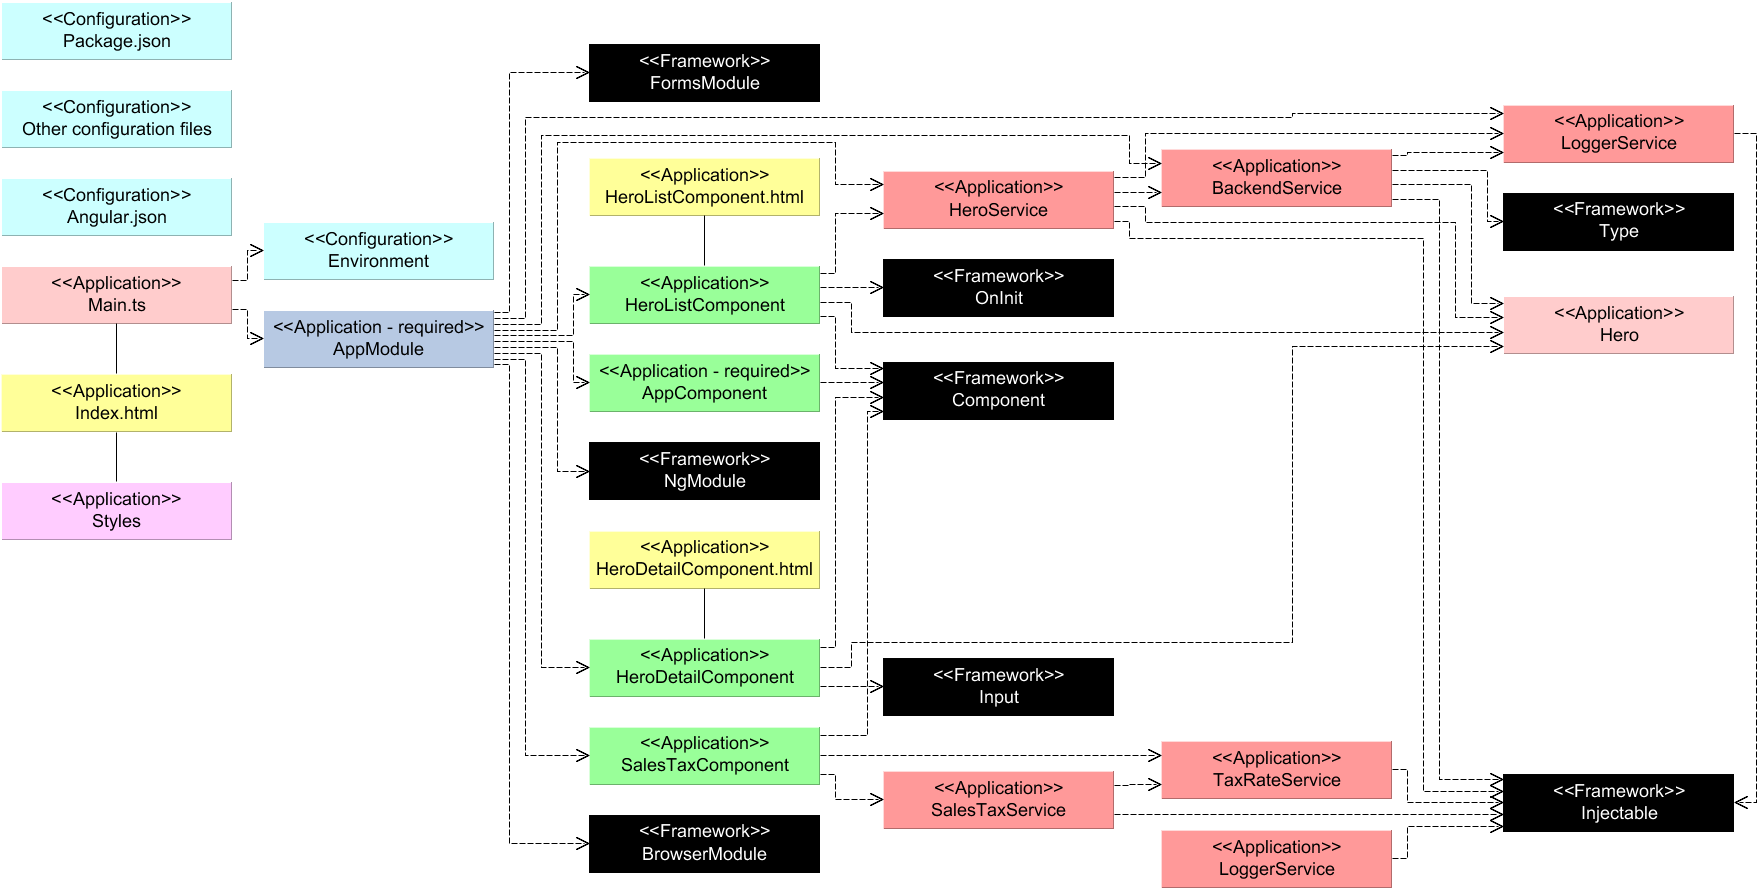
\includegraphics[width=14cm]{images/UMLDiagramExampleApp.png}
  \caption{Angular esimerkkisovelluksen luokkakaavio}
  \label{fig:UMLDiagramExampleApp}
\end{figure}

Sovelluskohtaisesti Angular-sovelluksen erikoistaminen tapahtuu metadatan ja dekoraattorien avulla. Sekä komponenteilla, palveluilla että moduuleilla on jokaisella oma dekoraattori. Esimerkiksi \mintinline{JavaScript}{@Component}-dekoraattorilla määritellään Angular-sovelluksessa tavallisesta JavaScript-luokasta komponentti \cite{ArchitectureComponents}. \mintinline{JavaScript}{@Component}-dekoraattorin metadatan avulla määritellään muun muassa, mitä palveluita komponenttiin injektoidaan ja mitä templaattia komponentti käyttää \cite{ArchitectureComponents}. 

Esimerkissä \ref{lst:SalesTaxComponent} on esitelty SalesTaxComponent-komponentti \cite{ExampleApplication}. \mintinline{JavaScript}{@Component}-dekoraattorilla määritellään riveillä 5 ... 17 metadata, jonka avulla \mintinline{JavaScript}{SalesTaxComponent}-luokasta tehdään Angular-komponentti. Metadatassa määritellään muun muassa, että \mintinline{JavaScript}{SalesTaxService}- ja \mintinline{JavaScript}{TaxRateService}-palvelut injektoidaan riippuvuusinjektion avulla \mintinline{JavaScript}{SalesTaxComponent}-komponenttiin. Lisäksi \mintinline{JavaScript}{@Component}-dekoraattorissa on määritelty \mintinline{JavaScript}{SalesTaxComponent}-komponentin templaatti riveillä 7 ... 15. 

\begin{lstlisting}[style=htmlcssjs, caption=SalesTaxComponent-komponentti \protect\cite{ExampleApplication}, label=lst:SalesTaxComponent ]
import { Component }       from '@angular/core';
import { SalesTaxService } from './sales-tax.service';
import { TaxRateService }  from './tax-rate.service';

@Component({
  selector:    'app-sales-tax',
  template: `
    <h2>Sales Tax Calculator</h2>
    <label>Amount: <input #amountBox (change)="0"></label>

    <div *ngIf="amountBox.value">
    The sales tax is
     {{ getTax(amountBox.value) | currency:'USD':true:'1.2-2' }}
    </div>
  `,
  providers: [SalesTaxService, TaxRateService]
})
export class SalesTaxComponent {
  constructor(private salesTaxService: SalesTaxService) { }

  getTax(value: string | number) {
    return this.salesTaxService.getVAT(value);
  }
}
\end{lstlisting}

Pitäisikö tähän vielä lisätä "kutakin aliluokkaryhmää kohti" yksi esimerkki --> eli moduuli ja service

Kontrollin kulku sovelluksessa --> Todo: Sekvenssikaavio: sis. datan tuleminen backendiltä frontille async-kutsulla (reducers), käyttäjä muuttaa usernamea palvelussa (two-way-data-binding esimerkki)

\section{Kehyksen arviointi}

Kehyksen arviointi - hyvät ja huonot puolet tässä esille

\subsection{Laatuskenaariot}

Laatuskenaariot


\section{Yhteenveto}

Yhteenveto



% Viitataan kuvaan \ref{fig:kaavio5}.
% \begin{figure}[H]
%   \centering
%   
\includegraphics[width=14cm]{images/kaavio5}
%   \caption{Kuvateksti}
%   \label{fig:kaavio5}
% \end{figure}


% --- References ---
%
% bibtex is used to generate the bibliography. The babplain style
% will generate numeric references (e.g. [1]) appropriate for theoretical
% computer science. If you need alphanumeric references (e.g [Tur90]), use
%
% \bibliographystyle{babalpha-lf}
%
% instead.


%\bibliographystyle{babplain-lf}
% \newpage
\bibliographystyle{apacite}
\renewcommand{\BRetrieved}[1]{Tarkistettu {#1}, saatavilla\ }
\renewcommand{\BRetrievedFrom}{Tarkistettu saatavilla\ }
\bibliography{references-fi}

% --- Appendices ---

% uncomment the following

% \newpage
% \appendix
% 
% \section{Esimerkkiliite}

\end{document}
